% https://www.youtube.com/watch?v=IZwU7jk3ITo&list=PLa_2246N48_rk8nzKg6VDykSEU6svwv4r&index=5

\documentclass{beamer}
\usetheme{Frankfurt}
\setbeamercovered{transparent}
\usepackage[utf8]{inputenc}
\usepackage{multimedia}        % Os recursos de vídeo podem não funcionar dependendo do leitor de PDF usado para abrir o vídeo (e.g., o Foxit não abre vídeo)

\title{Titulo}
\subtitle{Subtitulo}
\author[A.]{Autor}
\date{Data}
\institute[Inst.]{Intituição}
\logo{Imagem de logo}

\begin{document}

\begin{frame}
	\titlepage
\end{frame}


\begin{frame}
	\frametitle{Título Quadro 1}
	\framesubtitle{Subtitulo quadro 1}

	\movie[width=160px, height=90px]{Vídeo incorporado (depende do leitor de PDF)}{midia/latest_512_0193.mp4}

	\movie[width=160px, height=90px, externalviewer]{Vídeo externo}{midia/latest_512_0193.mp4}
\end{frame}

\begin{frame}
	\frametitle{Título Quadro 2}
	\framesubtitle{Vídeo com miniatura}
	
	\movie[width=160px, height=90px, poster]{1° frame (depende do leitor de PDF)}{midia/latest_512_0193.mp4} \\
	
	Miniatura \\
	\movie[width=160px, height=90px, externalviewer]{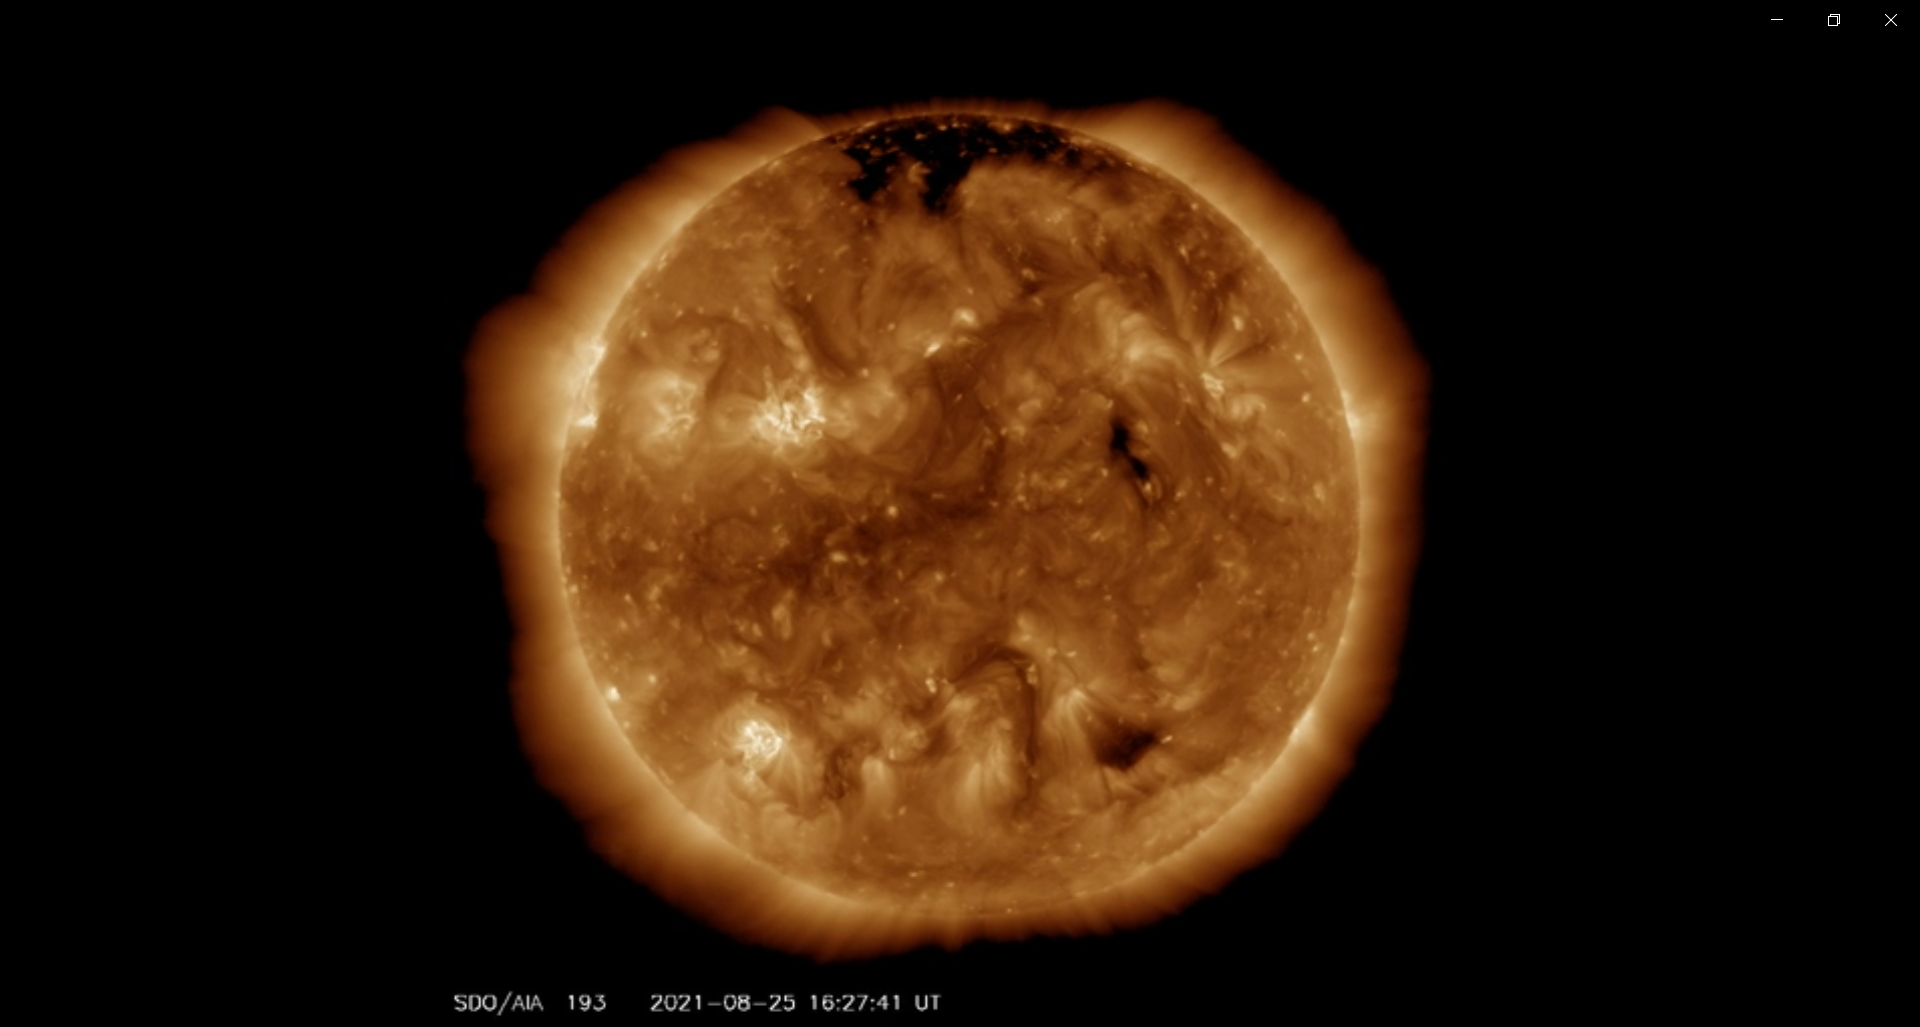
\includegraphics[width=160px, height=90px]{midia/mini_latest_512_0193.png}}{midia/latest_512_0193.mp4}
\end{frame}

\begin{frame}
	\frametitle{Título Quadro 3}
	\framesubtitle{Vídeo com comandos - funciona só quando o leitor aceita vídeo incorporado}
	
	\begin{center}
	\movie[width=160px, height=90px, loop]{Vídeo em loop}{midia/latest_512_0193.mp4}
	
	\movie[width=160px, height=90px, showcontrols]{Vídeo com barra de controles}{midia/latest_512_0193.mp4}
	\end{center}
\end{frame}

\begin{frame}
	\frametitle{Título Quadro 4}
	\framesubtitle{Áudio}
	
	\begin{center}
		\sound[externalviewer]{Tocar (depende do leitor de PDF)}{midia/burro.mp3}
	\end{center}
\end{frame}

\begin{frame}
	\frametitle{Título Quadro 5}
	\framesubtitle{Transição}
	
	\textbf{Obs.:} Foxit não executa as transições automaticamente
	\begin{itemize}
		\animate<2-3>
		 \item<1->	Slide 1
		 \item<2->	Slide 2
		 \item<3->	Slide 3
		 \item<4->	Slide 4
 	\end{itemize}
\end{frame}


\newcount{\nomeContador}
\newdimen{\nomeDimensao}
\begin{frame}
	\frametitle{Título Quadro 6}
	\framesubtitle{Transição com contador}
	
	\textbf{Obs.:} Foxit não executa as transições automaticamente
	
	\animate<2-3>
	\animatevalue<1-4>{\nomeContador}{0}{100}
	\animatevalue<1-4>{\nomeDimensao}{0cm}{8cm}
	
	\textcolor{red! \the\nomeContador !black}{Texto que muda de cor gradativamente (preto para vermelho)}
	
	{\hspace{\nomeDimensao}Texto que muda de posição}
	
\end{frame}

\begin{frame}
	\frametitle{Título Quadro 7}
	\framesubtitle{Transição com efeito}
	
	\textbf{Obs.:} Esse o Foxit executa, mas com transição manual
	
	\transdissolve[duration=0.5]<2>
	\begin{itemize}
		\item<1-> Slide 1
		\item<2-> Slide 2
		\item<3-> Slide 3
		\item<4-> Slide 4
	\end{itemize}
\end{frame}

\begin{frame}
	\frametitle{Título Quadro 8}
	\framesubtitle{Transição com efeito}
	
	\textbf{Obs.:} Esse o Foxit executa, mas com transição manual
	
	\transblindsvertical
	\begin{itemize}
		\item<1-> Slide 1
		\item<2-> Slide 2
		\item<3-> Slide 3
		\item<4-> Slide 4
	\end{itemize}
\end{frame}

\begin{frame}
	\frametitle{Título Quadro 9}
	\framesubtitle{Transição com efeito}
	
	\textbf{Obs.:} Esse o Foxit não executa
	
	\transwipe[direction=90]
	\begin{itemize}
		\item Slide 1
		\item Slide 2
		\item Slide 3
		\item Slide 4
	\end{itemize}
\end{frame}

\end{document}